%%%%%%%%%%%%%%%%%%%%%%%%%%%%%%%%%%%
\subsection{Thermometers}
\label{sec:fdsp-slow-cryo-therm}
% anselmo, jelena,

As mentioned above, a detailed 3D temperature map is important to monitor the correct functioning of the cryogenic system and the LAr uniformity.
Given the complexity and size of purity monitors, those can only be installed on the cryostat sides to provide a local measurement of
the LAr purity. While a direct measurement of the LAr purity across the entire cryostat is not viable, a sufficiently detailed 3D temperature map
can be used to predict the LAr purity using CFD simulations. Specially important is the vertical coordinate since this will be closely related to
the LAr recirculation and uniformity. 

High precision temperature sensors will be distributed near the TPC walls in two ways:
i) forming high density (>2 sensors/m) vertical arrays (the so-called T-gradient monitors), and ii) in coarser ($\sim$ 1 sensor/5 m) 2D arrays 
at the top and bottom of the detector, which are the most delicate regions (the so-called individual sensors).   

Since temperature variations inside the cryostat are expected to be very small ($0.02 K$), to properly measure the 3D temperature map 
sensors must be cross-calibrated to better than $0.005 K$. Most sensors will be calibrated in the laboratory, prior to installation,
as described in the next section. This is in fact the only viable method for sensors behind the APAs and top/bottom of the detector since the available space is restricted.  
Given the precision required and the unknown longevity of the sensors (which could require a new calibration after some time), and complementary method
will be used for T-gradient monitors behind the front end-walls. In those areas there is sufficient space for a movable system, which can be used to cross-calibrate insitu
the temperature sensors. This calibration method is described in the section about dynamic T-gradient monitors. 

In the baseline design for all three systems mentioned above three elements are common: the sensor model, the cable model and the readout system.
Platinum sensors with \SI{100}{\ohm} resistance (PT100 series), produced by Lakeshore will be used. 
This choice is adequate for the temperature range of interest, 83-92\si{K}, since in this range those sensors have high reproducibility
of just \SI{5}{mK} and absolute temperature accuracy of \SI{100}{mK}.
In addition, the plan is to use the 4-wire readout greatly reducing the issues related to the lead resistance, any parasitic resistances,
connections through the flange and general electromagnetic noise pick-up. The Lakeshore PT102 sensors have being previously used in the 35t prototype and ProtoDUNE SP detector,
giving excellent results. As shown in Fig.~\ref{fig:sensor_cable}, the PT102 sensor has a length of \SI{21}{mm}, which can easily be accommodated in the DUNE T-gradient monitors. 

\begin{dunefigure}[diag PT102]{fig:sensor_cable}
  {DUNE baseline choices for sensor and cable. Left: Schematic diagram of the PT102 sensor from the Lakeshore company. Right: Schematic diagram and properties of the four wires cable from the
  Axon company}
  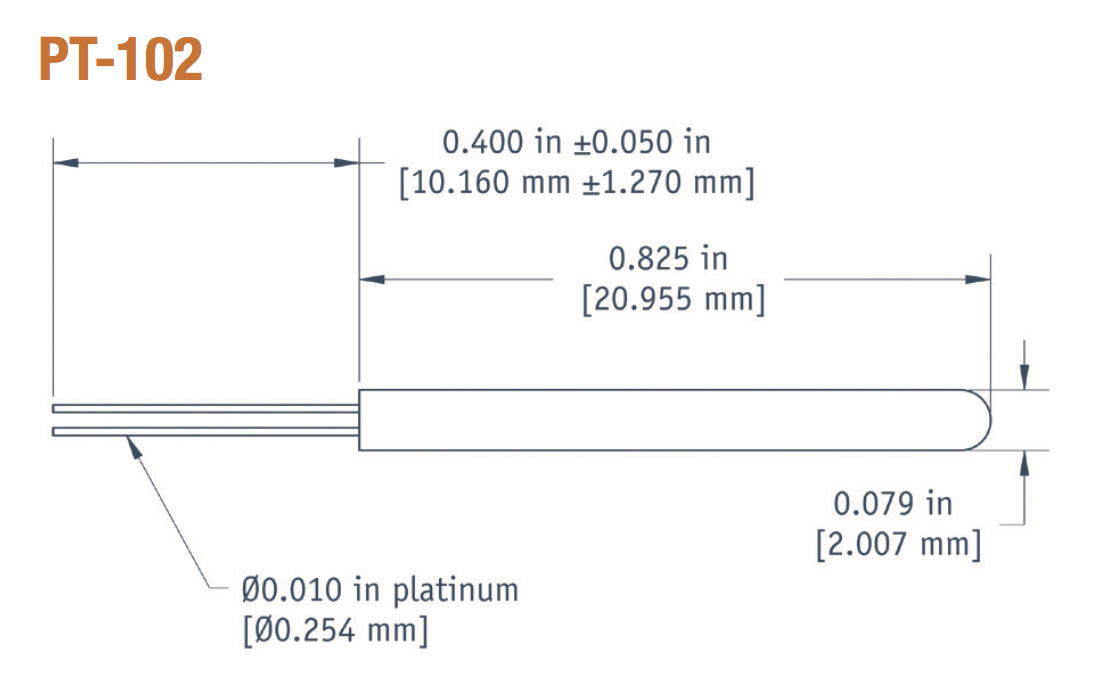
\includegraphics[width=0.4\textwidth]{cisc_pt102.png}
  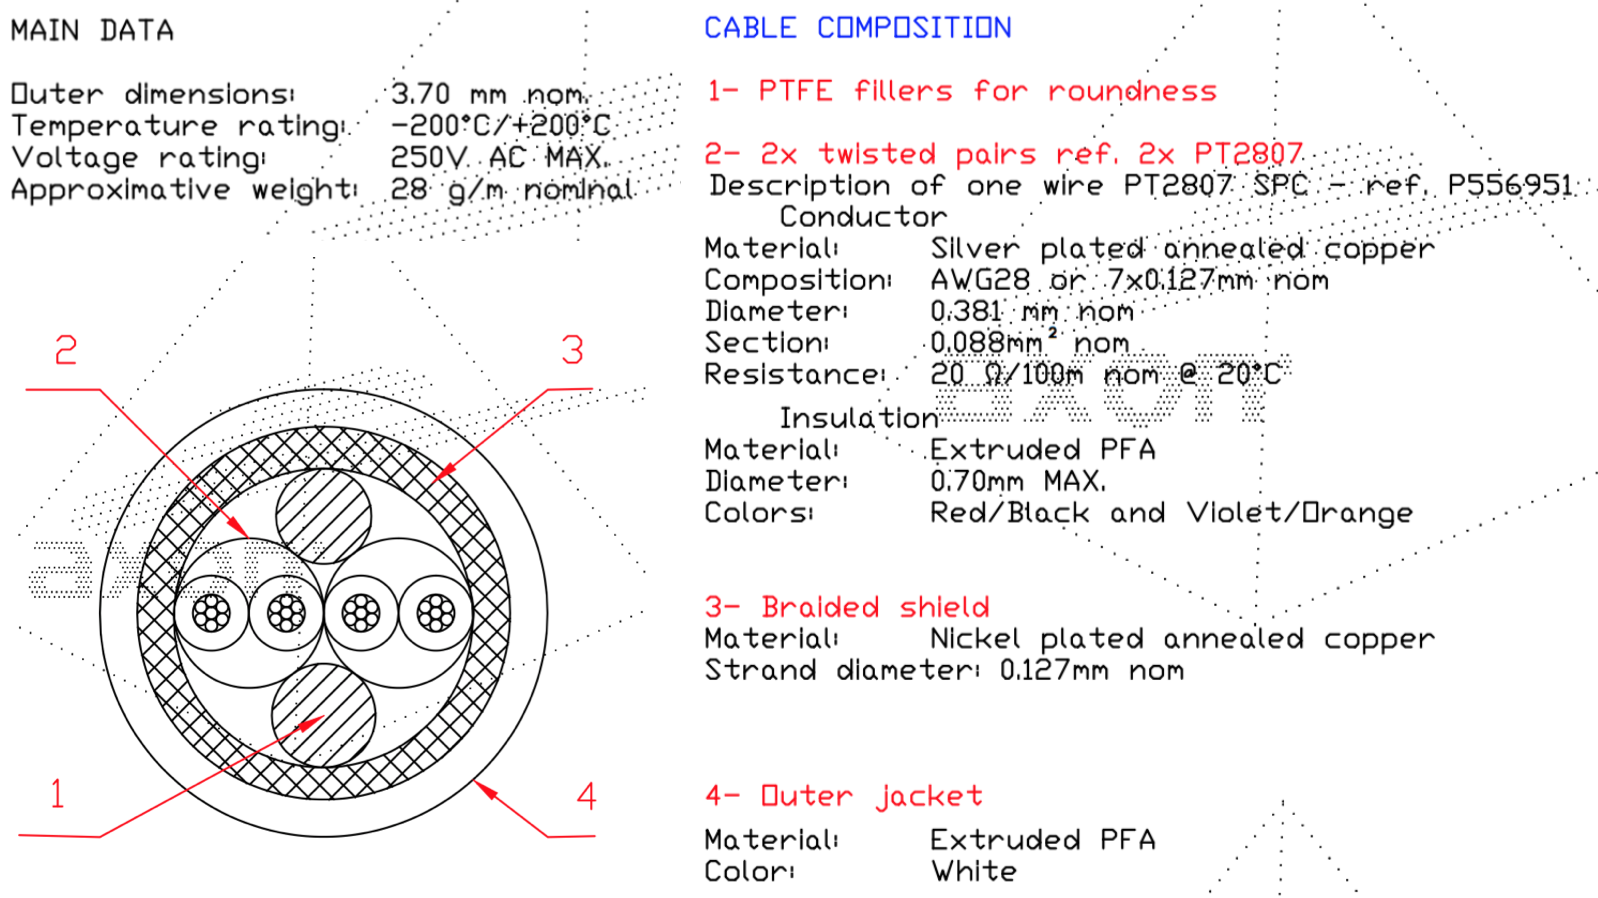
\includegraphics[width=0.55\textwidth]{cisc_TAxonCable.png}
\end{dunefigure}

For the readout cables a custom cable made by Axon is the baseline. It consists in four teflon-jacketed 
cupper wires (AWG28), forming two twisted pairs, with an metalic external shield
and an outer teflon jacket. Further details are given in Fig.~\ref{fig:sensor_cable}-Right. 
The readout system will be described below in a separate subsection. 

Another set of lower precision sensors will be also used to monitor the filling of the cryostat in its initial stage. Those sensors will be epoxied into the cryostat bottom membrane with
a density to be determined, which will not exceed 1 sensor every 5 m. 
Finally, the inner walls and roof of the cryostat will be instrumented with the same type of sensors in order to monitor their temperature during cooldown and filling.
The baseline distribution would be three vertical arrays of sensors: one in each side of the cryostat behind the end walls and another one in the middle behind the APAs. 

except for the membrane sensors that may come from Minco.

% % % %
\subsubsection{Static T-Gradient monitors}

Several vertical arrays of high precision temperature sensors cross-calibrated in the laboratory will be installed behind the APAs.
Since the electric potential in this area is zero no electric field shielding is required, simplifying enormously the mechanical design.

Sensors are cross-calibrated in the lab using a well controlled environment and a high precission readout system, described below in a separate subsection.
Although the calibration procedure will certainly improve, the one currently use for ProtoDUNE-SP is descrived here.
Four sensors are placed as close as possible (such that identical temperature can be assumed for all of them) inside a small cylyndrical aluminum capsule,
which helps in minimizing convection. One of the sensors acts as reference while the other three are the ones being calibrated. Five independent calibrations
are performed for each set of three sensors, such that the reproducibility of each sensor can be computed. For each calibration 
the capsule is introduced in a PLA box of size 9.5x9.5x19 $cm^3$, with two concentrical independent volumes of LAr
and sourounded by a polystire box with 15 cm thick walls. A small quantity of LAr is used to cooldown the capsule to $~90 K$. Then the capsule is covered by LAr such that it penetrates
inside fully covering the sensors. Once the temperature stabilizes to the 1-2 mk level (after 5-15 minutes) measurements are taken. Then the capsule is taken out from LAr
and kept at room temperature until it reaches 200 K. As mentioned above, this procedure is repeated five times, before going to the next set of three sensors.  
As shown in Figure ~\ref{fig:Trepro} a reproducibility of $\sim2 mk$ has being achieved in ProtoDUNE-SP. 

The baseline design for the mechanics of the system is shown in Fig.~\ref{}. It consists in two stainless strings anchored at top and bottom corners of the cryostat
using M10 bolts. One of the strings is used to route the cables while the other serves as support for temperature sensors. The need of intermediate anchoring points is under discussion. 


The four wires of each cable will be soldered to the inner pins of male SUBD-25 connectors on the flanges. 

\begin{dunefigure}[sensor support]{fig:sensor-support}
  {Lakeshore PT102 sensor mounted on a PCB with an IDC-4 connector}
  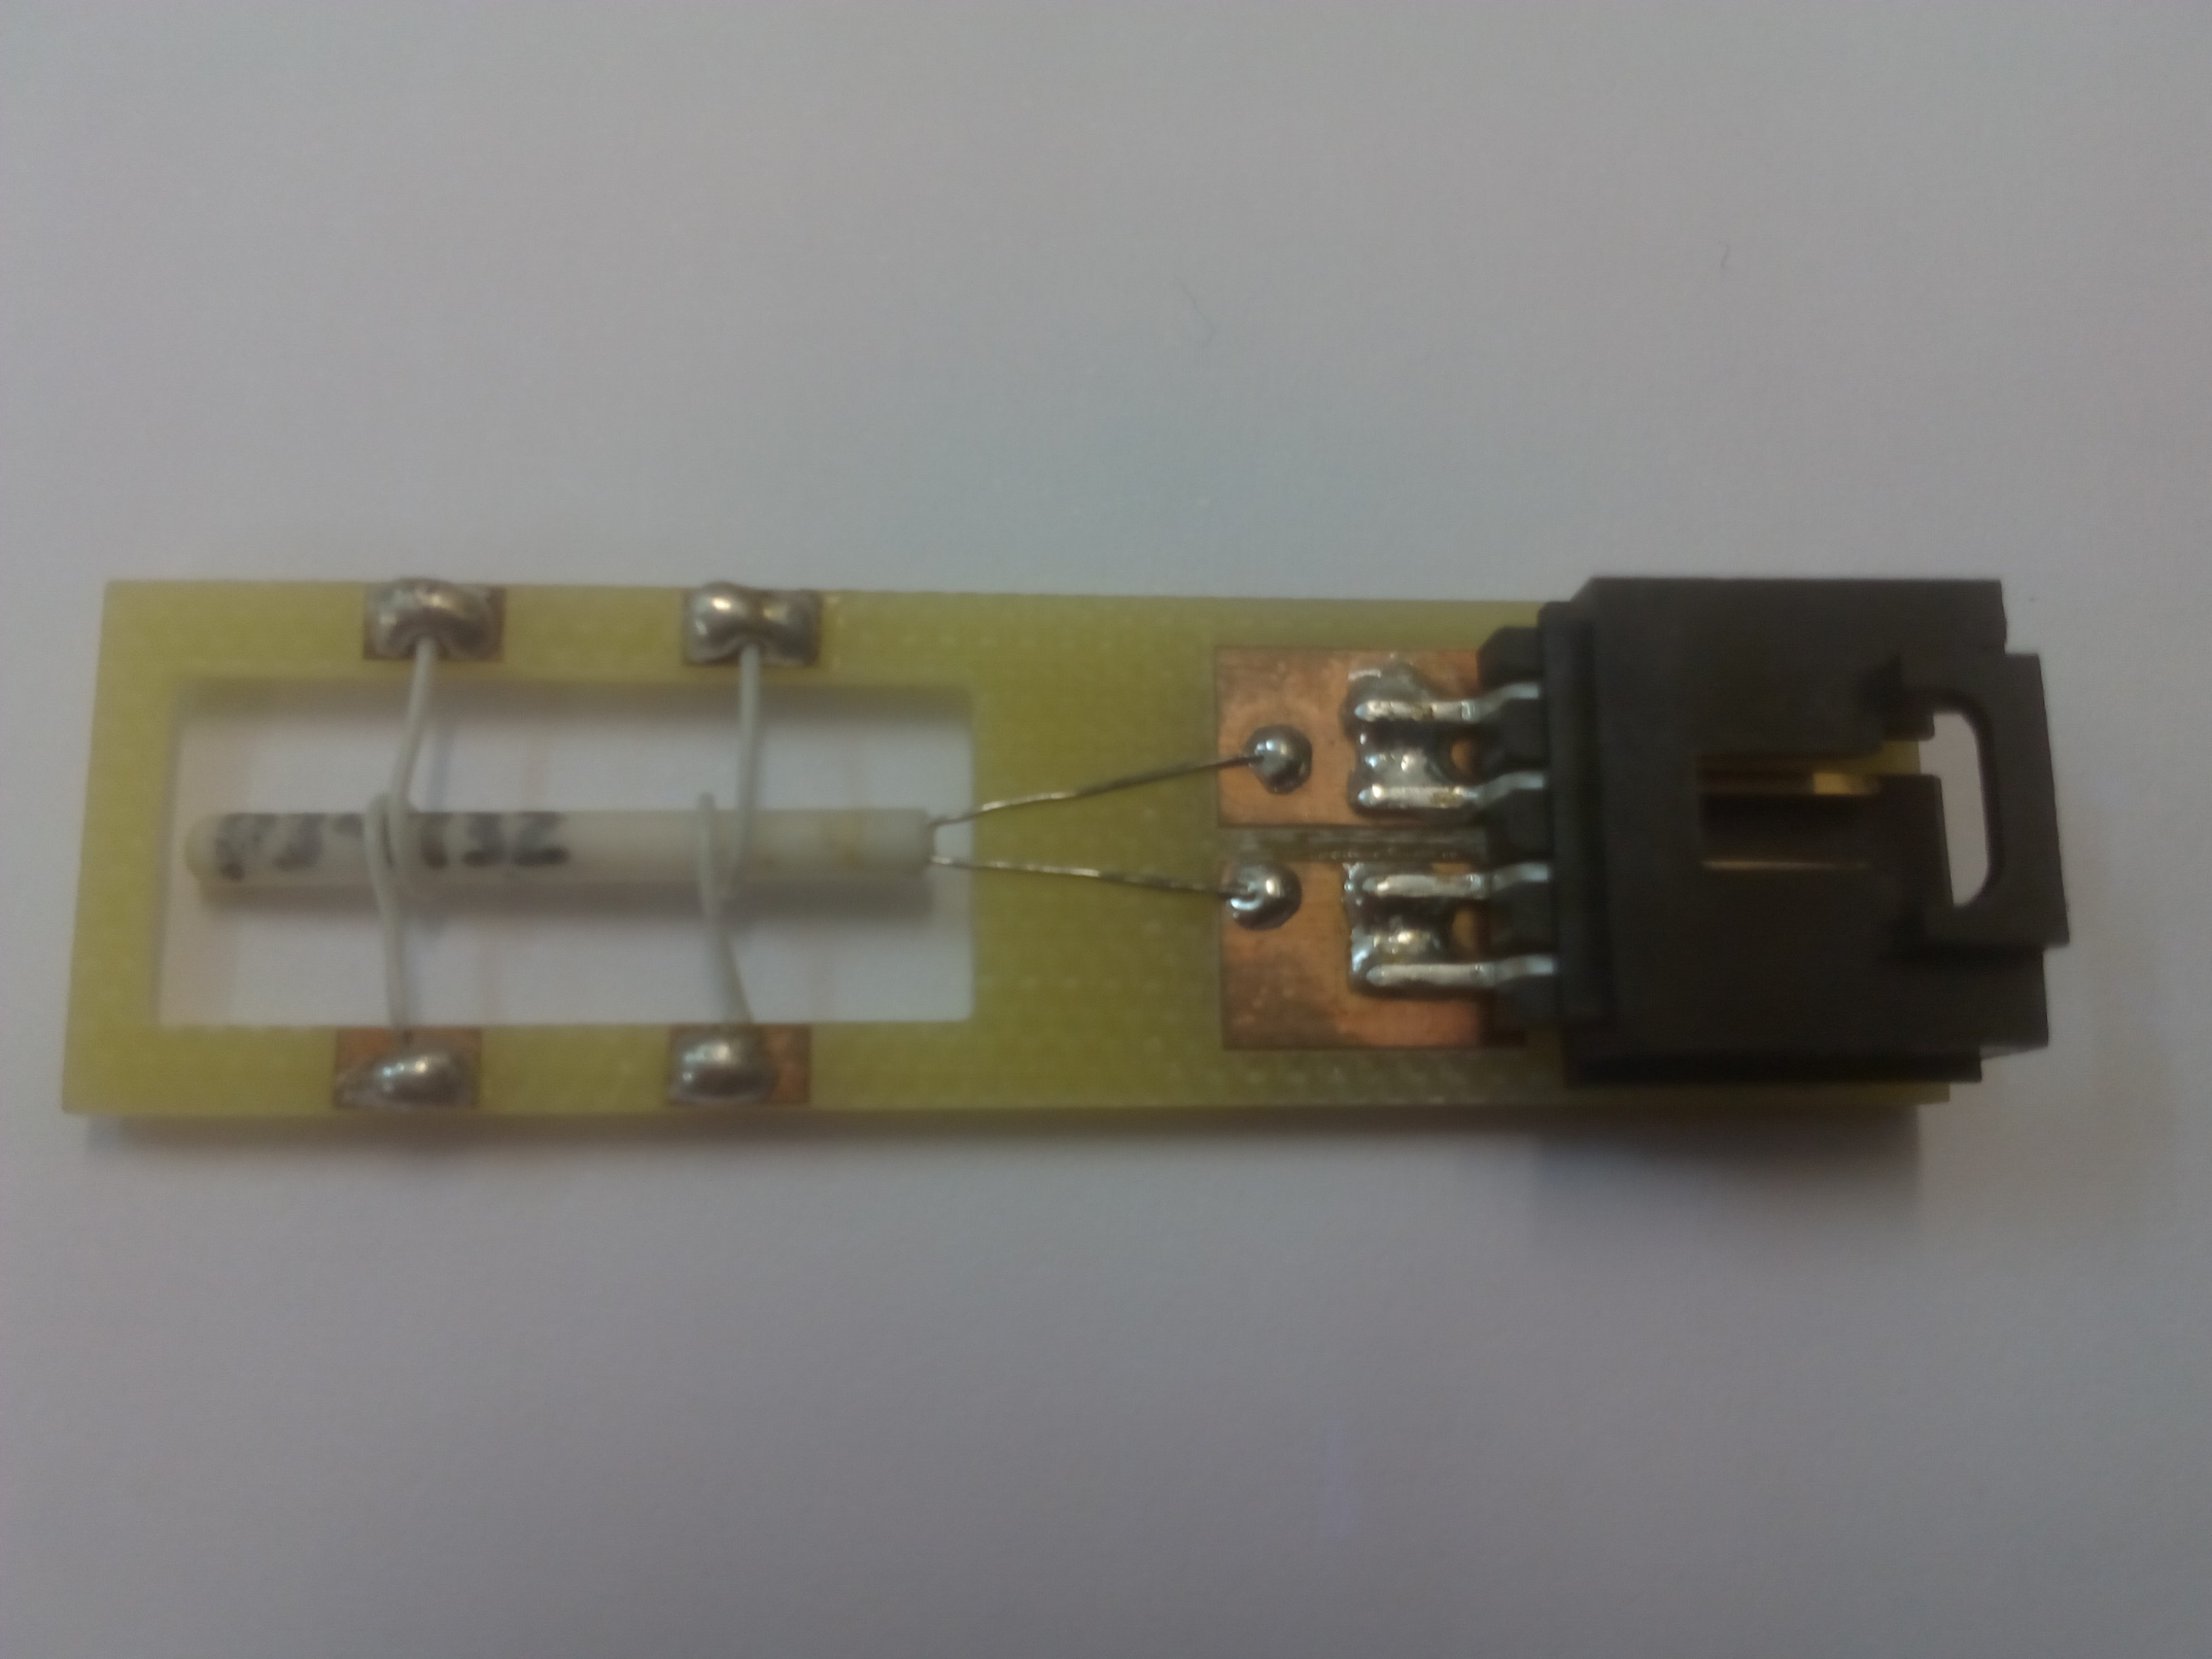
\includegraphics[width=0.3\textwidth]{cisc_TsensorSupport.jpg}%
\end{dunefigure}


\begin{dunefigure}[sensor support]{fig:Trepro}
  {Temperature offset between two sensors as a function of time for five independent inmersions in LAr. The reproducibility is $\sim 2 mk$,
    defined as the RMS of the mean offset in the flat region}
  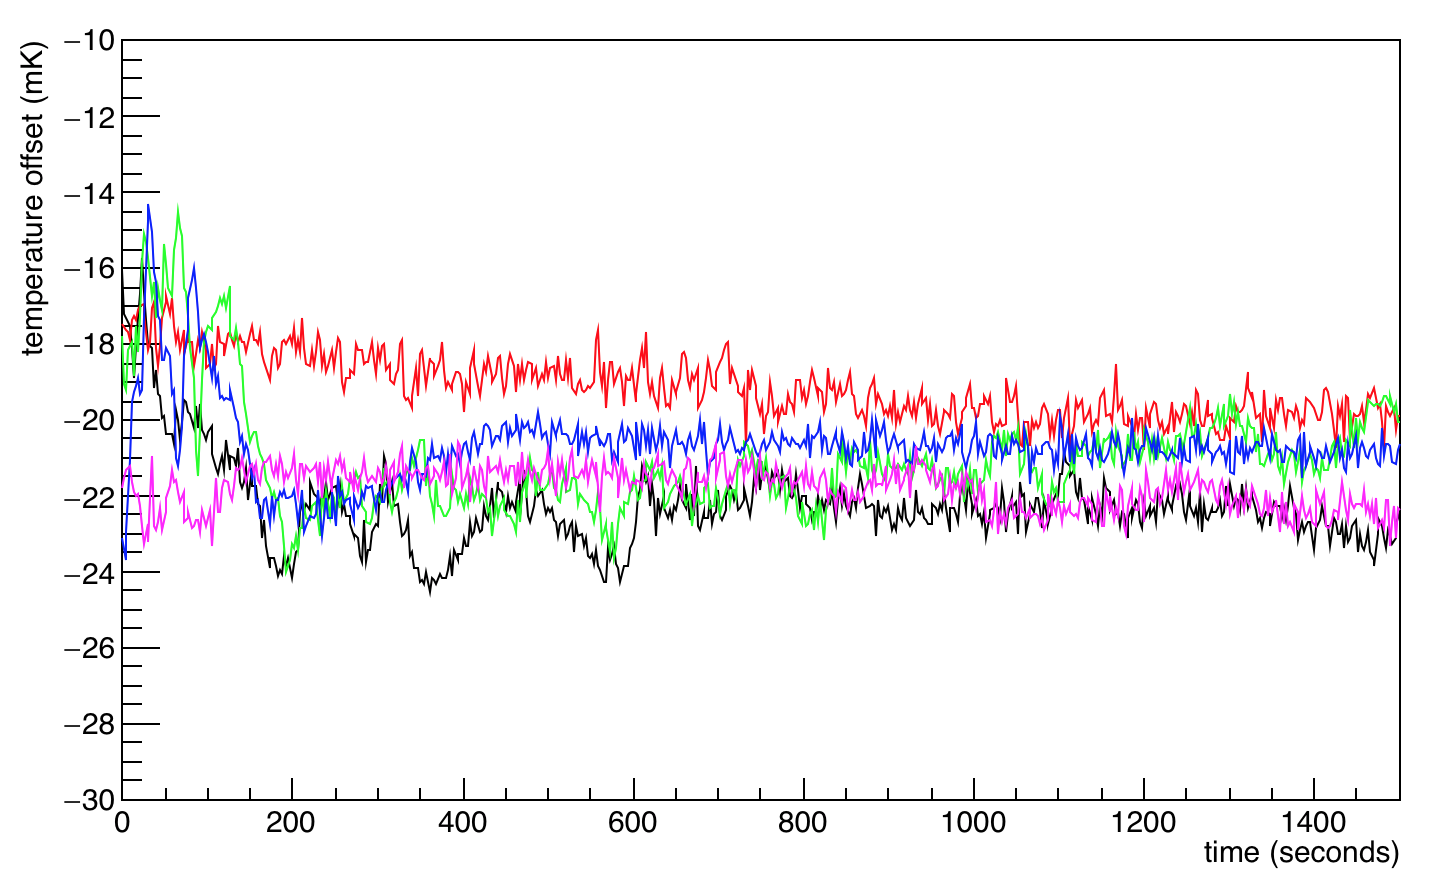
\includegraphics[width=0.5\textwidth]{cisc_Treproducibility.png}%
\end{dunefigure}


% % % %
\subsubsection{Dynamic T-Gradient monitors}

Dynamic temperature monitor is a vertical array of high precision temperature sensors with the goal of measuring vertical temperature gradient with precision of few mK. The design of the system is driven by two factors:
\begin{itemize}
\item
few mK uncertainty in the measured vertical temperature profile over the entire detector height is required to monitor LAr purity and provide useful feedback of efficiency cryogenic recirculation and purification.
\item
simulations of the cryogenic recirculation predict very slow change in temperature at meter scale except at the bottom and top of the cryostat. Thus, sensors will be placed every \SI{50}{cm} along the detector height with increased frequency in the first \SI{50}{cm}, closest to the bottom of the cryostat and the last \SI{50}{cm}, closest to the top of the cryostat, where spacing between sensors is reduced to \SI{10}{cm}.
 \end{itemize}


 In order to address concerns related to potential difference in the sensor reading prior to installation and after installation in DUNE FD dynamic temperature monitor allows cross-calibration of sensors in situ. Namely, this T-gradient monitor  can move vertically while installed in DUNE FD, which allows for precise cross-calibration between the sensors in-situ at predefined locations as well as in between them. The procedure for cross-calibrations is the following: the temperature reading is taken at the lowest position with all sensors. Then, the stepper motor moves the carrier rod up for \SI{50}{cm} putting all sensors in the location of their neighbor that is \SI{50}{cm} above them. Then the second reading is taken. In this manner, except for the lowest position we have temperature measurement at each location with two adjacent sensors, and by linking the temperature offsets between the two readings at each location, temperature readings from all sensors are cross-calibrated in situ, cancelling all offsets due to electromagnetic noise or any parasitic resistances that may have prevailed despite the four point connection to the sensors that should cancel most of the offsets. These measurements are taken with very stable current source, which ensures high precision of repeated temperature measurements over time. The motion of the dynamic T-monitor is stepper motor operated, delivering measurements with high spatial resolution. 

\subsubsection{Dynamic t-gradient monitor design}
Dynamic T-gradient monitor consists of three distinct parts: carrier rod on which sensors are mounted, enclosure above the cryostat housing the space that allows vertical motion of the carrier rod 1.5\,m above its lowest location, and motion mechanism. The motion mechanism consists of a stepper motor connected to a gear and pinion motion mechanism through ferrofluidic dynamic seal. The sensors have two pins that are soldered to a printed circuit board (PCB). Two wires are soldered to the common soldering pad for each pin, individually.   There is a cutout in the PCB around the sensor that allows free flow of argon for more accurate temperature reading.  Stepper motors typically have very fine steps allowing high precision positioning of the sensors.  Figure~\ref{fig:DT_design} shows the overall design of the dynamic T-gradient monitor with the sensor carrier rod, enclosure above the cryostat and stepper motor mounted on the side of the enclosure. The enclosure consists of two parts connected by 6-cross flange. One side of the 6-cross flange will be used to for the signal wires, another side will be used as a viewing window, while the two other ports will be spares. Figure~\ref{fig:sensonr_on_pcb_motor}-Left shows the mounting of the PCB board on the carrier rod and mounting on the sensor on the PCB along with the four point connection to the signal readout wires. Finally, Figure~\ref{fig:sensonr_on_pcb_motor}-Right shows the stepper motor mounted on the side of the rod enclosure. The motor is kept outside, at room temperature and its power and control cables are also kept outside.

\begin{dunefigure}[dyn-T-grad]{fig:DT_design}
  {An overview of the dynamic T-gradient monitor.}
 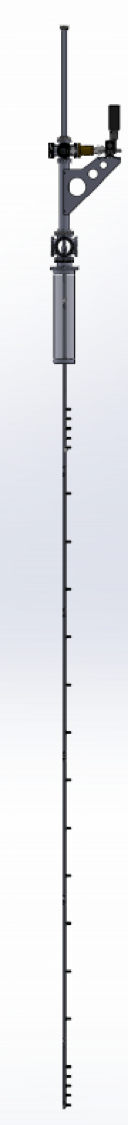
\includegraphics[width=0.11\textwidth,angle=90]{cisc_DTOverview.png}
\end{dunefigure}
\begin{dunefigure}[]{fig:sensor_on_pcb_motor}
  {Left: Sensor mounted on a PCB board and PCB board mounted on the rod. Right:
    The driving mechanism of the dynamic T-gradient monitor. It consists of a stepper motor driving the pinion and gear linear motion mechanism. }
  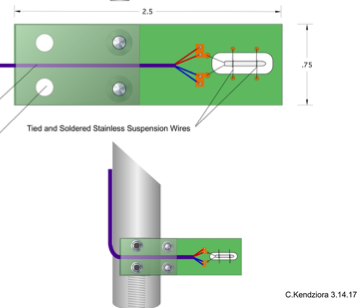
\includegraphics[width=0.40\textwidth]{cisc_DTSensorMount.png}
  \hspace{3cm}%
  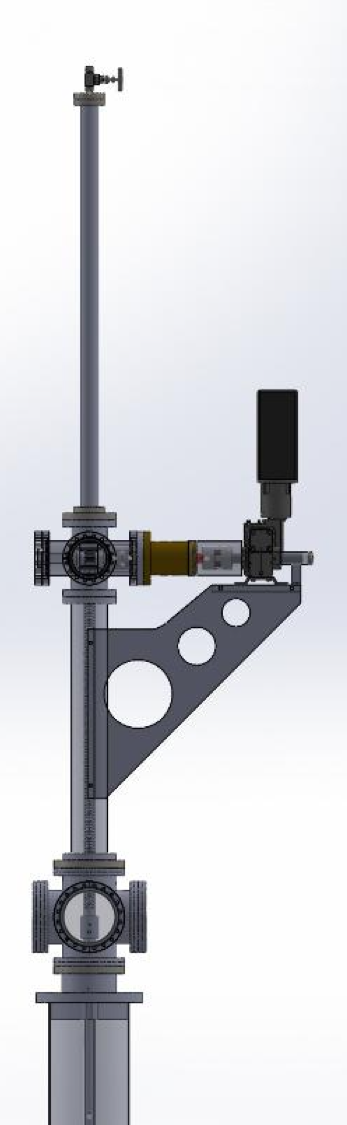
\includegraphics[width=0.12\textwidth]{cisc_DTMotor.png}
\end{dunefigure}

% % % %
\subsubsection{Individual Temperature Sensors}

T-Gradient monitors will provide a vertical temperature profiling outside the TPCs. Those will be complemented by a coarser 2D array at the top and bottom of the
detector. Sensors, cables and readout system will be the same as for the T-gradient monitors. 

In principle a similar distribution of sensors will be used at top and bottom.
Following ProtoDUNE-SP design, bottom sensors will use the cryogenic pipes as support structure, while top sensors will be anchored to the ground planes.
Teflon pieces (see Fig.~\ref{fig:cable-support}) will be used to route cables from the sensors to the DSS/cryogenic ports, which will be used to extract the cables.
The four wires of each cable will be soldered to the inner pins of male SUBD-25 connectors on the flanges. 

\begin{dunefigure}[sensorcable support]{fig:cable-support}
  {Left: support for two cables on ground planes. Right: Supports for three cables  mounted on cryogenics pipes using split clamps}
% This PDF is made from the .dot of the same name.
  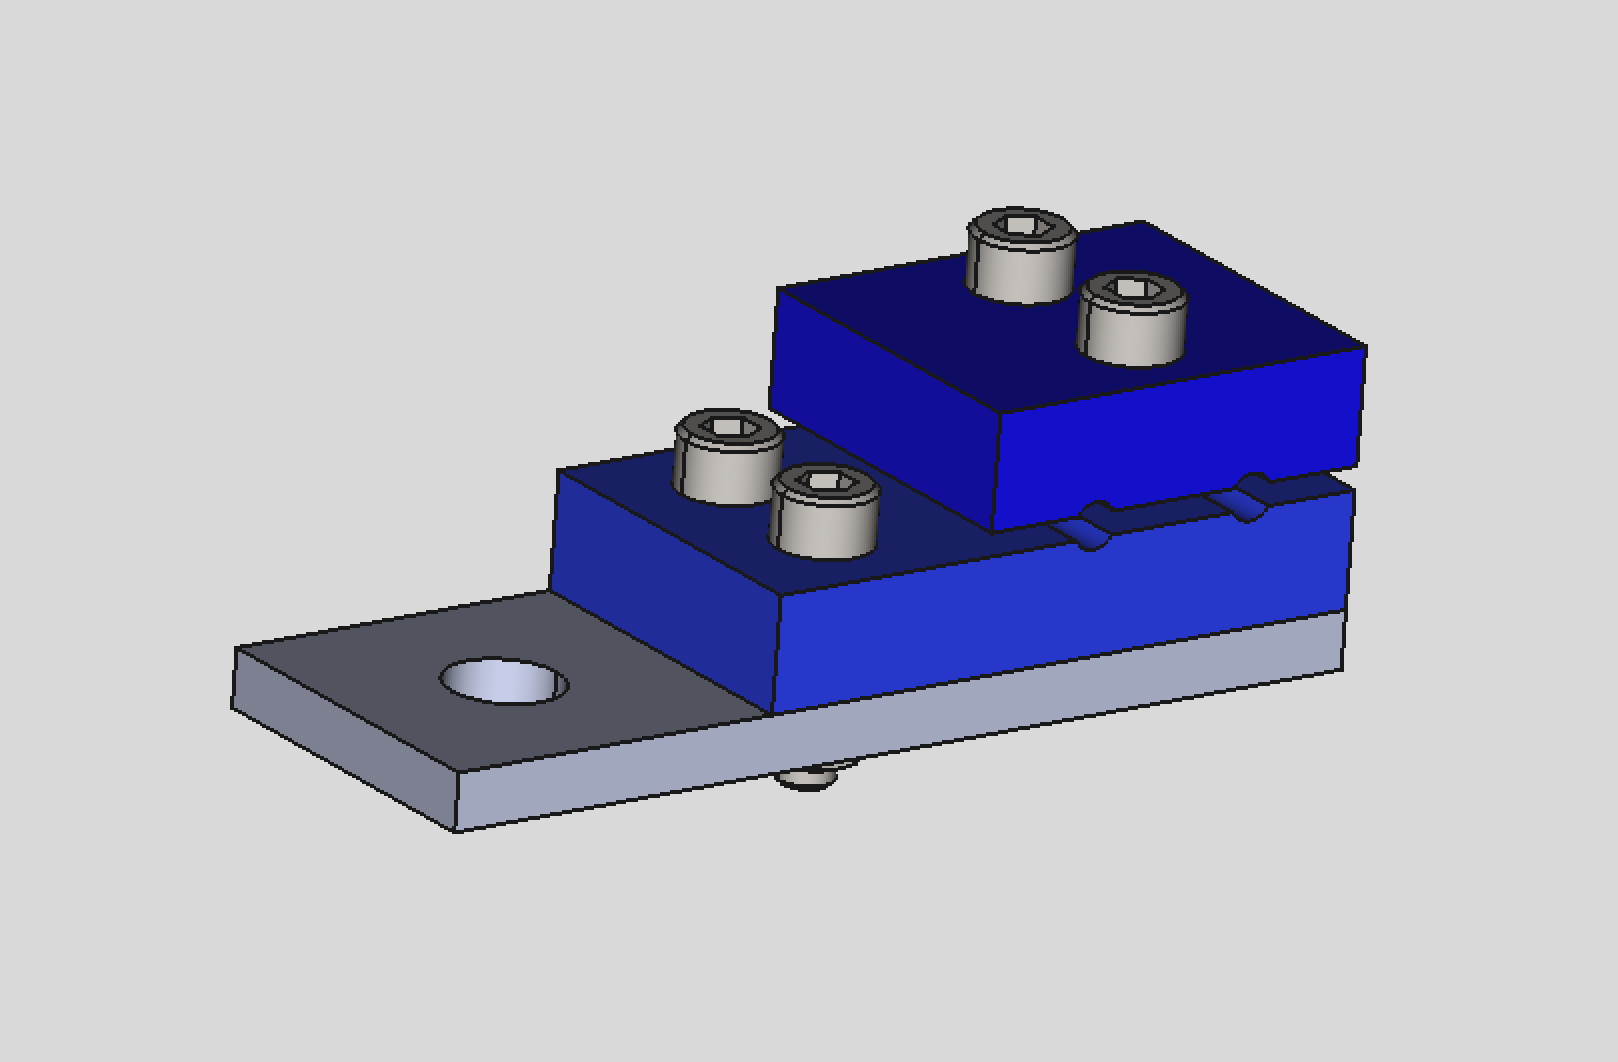
\includegraphics[width=0.3\textwidth]{cisc_TcableSupportGP.png}
  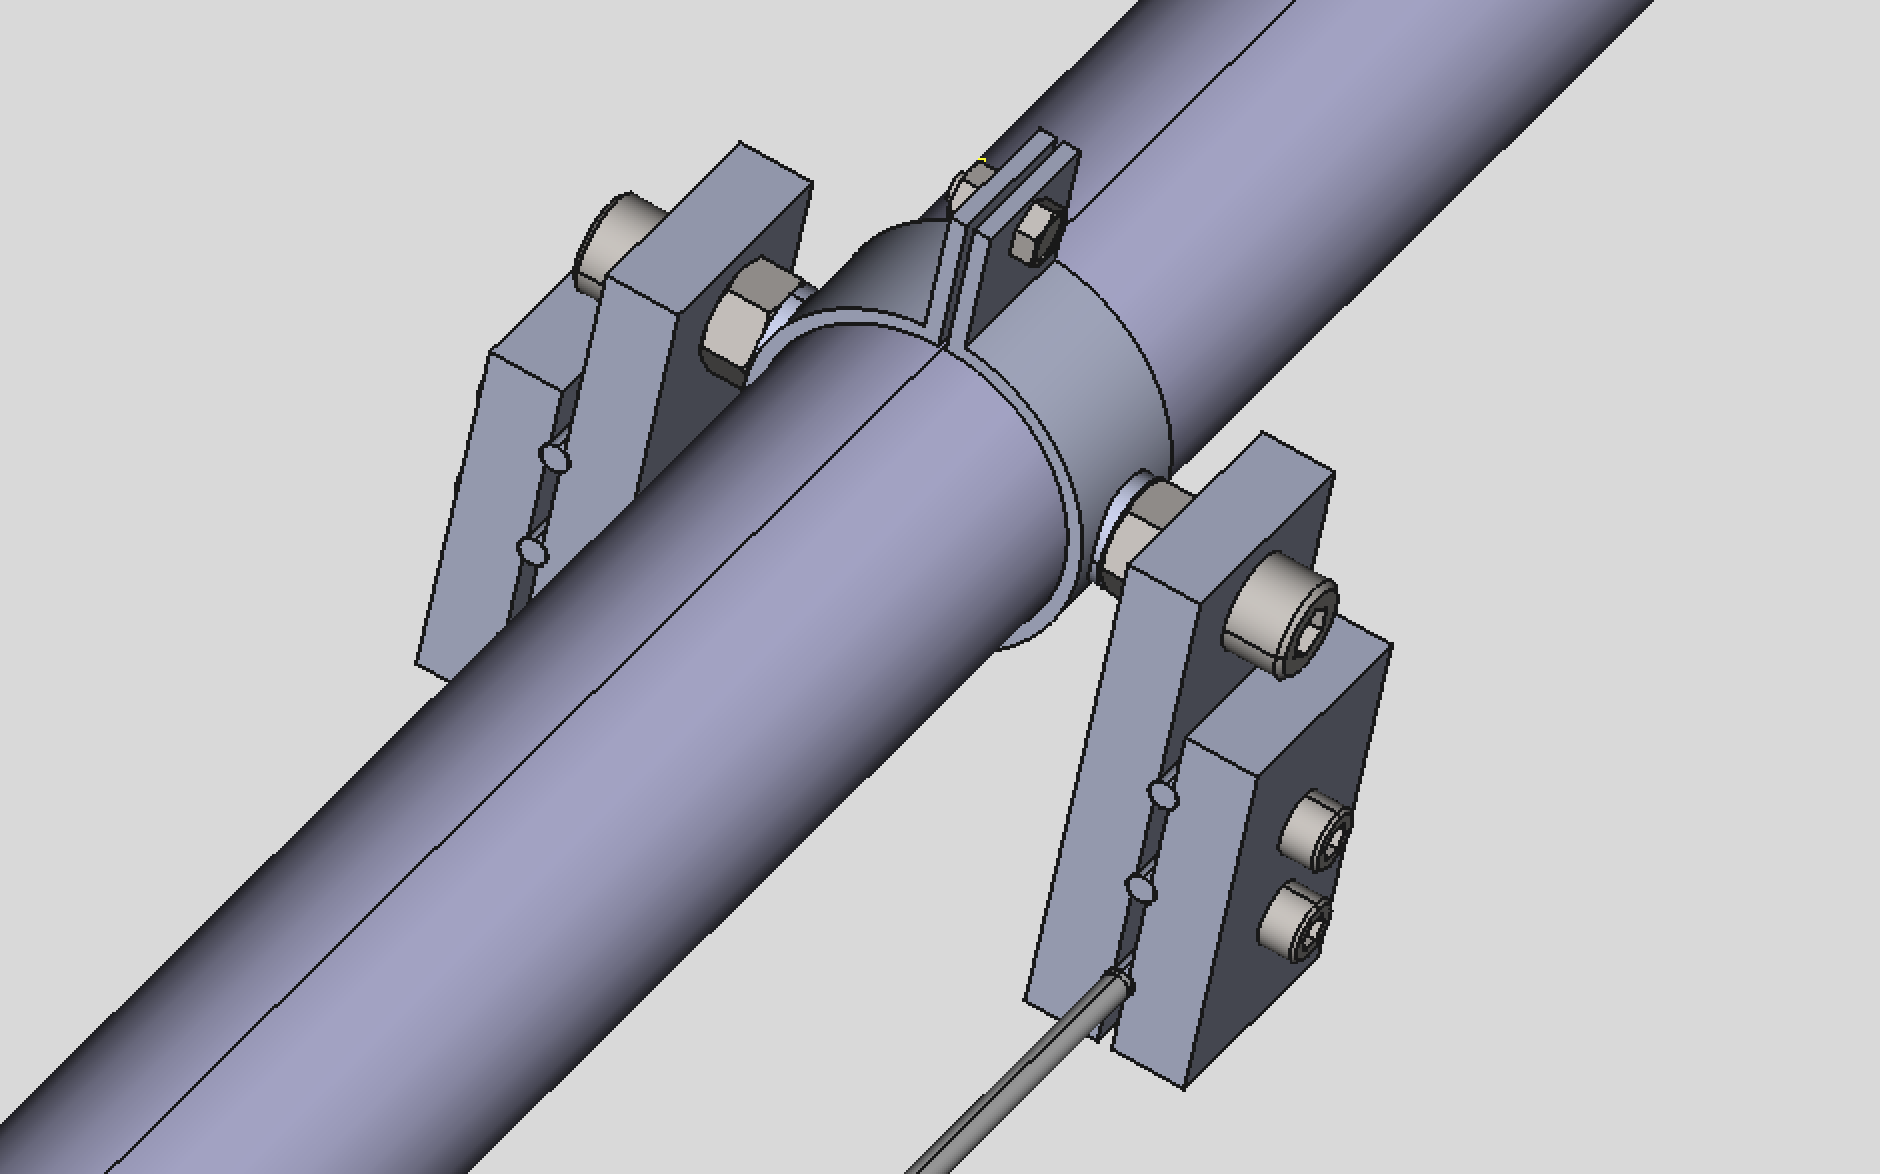
\includegraphics[width=0.315\textwidth]{cisc_TcableSupportPipes.png}
\end{dunefigure}


% % % %
\subsubsection{Readout system for thermometers}
\label{sec:fdsp-slow-cryo-therm-readout}

A high precision and very stable system is required to achieved the design precihsion of $< 5 mk$.
The proposed readout system is the one used in ProtoDUNE-SP, which is based on a variant of an existing mass PT100 temperature readout system developed at
CERN for one of the LHC experiments. The system consists of three parts:
\begin{itemize}
\item An accurate current source for the excitation of the temperature sensors, implemented by a compact electronic circuit using high a precision voltage reference from Texas Instruments. 
\item A multiplexing circuit based on an ADG707 Analog Device multiplexer electronic device;
\item A high resolution and accuracy voltage signal readout module based on National Instruments NI9238, which has 24 bits resolution over 1 Volt range.
  This module is inserted in a National Instruments Ethernet DAQ backplane, which will distribute the temperature values to the main Slow Control Software
  through the standard protocol, OPC UA. The Ethernet DAQ will include also the multiplexing logic.
\end{itemize}


The current mode of operation averages over 2000 samples taken in 1 second. 
As shown in Fig.~\ref{} the system has a resolution better than 1 mk.  


\fixme{add figure showing the resolution of the system}
